\documentclass{article}

\usepackage{fancyhdr}
\usepackage{extramarks}
\usepackage{amsmath}
\usepackage{amsthm}
\usepackage{amsfonts}
\usepackage{tikz}
\usepackage[plain]{algorithm}
\usepackage{algpseudocode}
\usepackage{physics}

\usetikzlibrary{automata,positioning}

%
% Basic Document Settings
%

\topmargin=-0.45in
\evensidemargin=0in
\oddsidemargin=0in
\textwidth=6.5in
\textheight=9.0in
\headsep=0.25in

\linespread{1.1}

\pagestyle{fancy}
\lhead{\hmwkAuthorName}
\chead{\hmwkClass\ (\hmwkClassInstructor\ \hmwkClassTime): \hmwkTitle}
\rhead{\firstxmark}
\lfoot{\lastxmark}
\cfoot{\thepage}

\renewcommand\headrulewidth{0.4pt}
\renewcommand\footrulewidth{0.4pt}

\setlength\parindent{0pt}

%
% Create Problem Sections
%

\newcommand{\enterProblemHeader}[1]{
    \nobreak\extramarks{}{Problem \arabic{#1} continued on next page\ldots}\nobreak{}
    \nobreak\extramarks{Problem \arabic{#1} (continued)}{Problem \arabic{#1} continued on next page\ldots}\nobreak{}
}

\newcommand{\exitProblemHeader}[1]{
    \nobreak\extramarks{Problem \arabic{#1} (continued)}{Problem \arabic{#1} continued on next page\ldots}\nobreak{}
    \stepcounter{#1}
    \nobreak\extramarks{Problem \arabic{#1}}{}\nobreak{}
}

\setcounter{secnumdepth}{0}
\newcounter{partCounter}
\newcounter{homeworkProblemCounter}
\setcounter{homeworkProblemCounter}{1}
\nobreak\extramarks{Problem \arabic{homeworkProblemCounter}}{}\nobreak{}

%
% Homework Problem Environment
%
% This environment takes an optional argument. When given, it will adjust the
% problem counter. This is useful for when the problems given for your
% assignment aren't sequential. See the last 3 problems of this template for an
% example.
%
\newenvironment{homeworkProblem}[1][-1]{
    \ifnum#1>0
        \setcounter{homeworkProblemCounter}{#1}
    \fi
    \section{Problem \arabic{homeworkProblemCounter}}
    \setcounter{partCounter}{1}
    \enterProblemHeader{homeworkProblemCounter}
}{
    \exitProblemHeader{homeworkProblemCounter}
}

%
% Homework Details
%   - Title
%   - Due date
%   - Class
%   - Section/Time
%   - Instructor
%   - Author
%

\newcommand{\hmwkTitle}{Assignment 3}
\newcommand{\hmwkDueDate}{February 12, 2024}
\newcommand{\hmwkClass}{COMP 4200}
\newcommand{\hmwkClassTime}{001}
\newcommand{\hmwkClassInstructor}{Professor Kwon}
\newcommand{\hmwkAuthorName}{\textbf{Matthew Rogers}}

%
% Title Page
%

\title{
    \vspace{2in}
    \textmd{\textbf{\hmwkClass:\ \hmwkTitle}}\\
    \normalsize\vspace{0.1in}\small{Due\ on\ \hmwkDueDate}\\
    \vspace{0.1in}\large{\textit{\hmwkClassInstructor\ \hmwkClassTime}}
    \vspace{3in}
}

\author{\hmwkAuthorName}
\date{}

\renewcommand{\part}[1]{\textbf{\large Part \Alph{partCounter}}\stepcounter{partCounter}\\}

%
% Various Helper Commands
%

% Useful for algorithms
\newcommand{\alg}[1]{\textsc{\bfseries \footnotesize #1}}

% For derivatives
\newcommand{\deriv}[1]{\frac{\mathrm{d}}{\mathrm{d}x} (#1)}

% For partial derivatives
\newcommand{\pderiv}[2]{\frac{\partial}{\partial #1} (#2)}

% Integral dx
\newcommand{\dx}{\mathrm{d}x}

% Alias for the Solution section header
\newcommand{\solution}{\textbf{\large Solution}}

% Probability commands: Expectation, Variance, Covariance, Bias
\newcommand{\E}{\mathrm{E}}
\newcommand{\Var}{\mathrm{Var}}
\newcommand{\Cov}{\mathrm{Cov}}
\newcommand{\Bias}{\mathrm{Bias}}

\begin{document}

\maketitle

\pagebreak

\begin{homeworkProblem}
    Construct NFAs that recognize the following languages:

    \begin{enumerate}
        \item All binary numbers that contain a 1 in the 3rd location from the right.
        \item All binary numbers that contain at most two 1's or contain at most two 0's.
        \item All binary numbers that can be divided by 4.
    \end{enumerate}

    \textbf{Solution}
    \\
    \\
    \textbf{Part One}

    \begin{figure}[h]
        \centering
        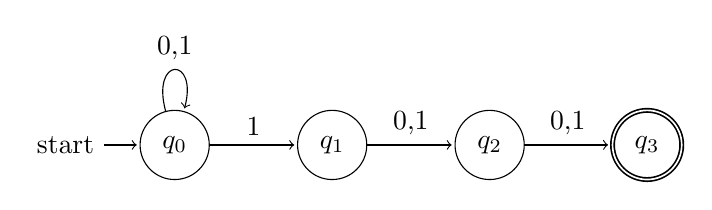
\begin{tikzpicture}[shorten >=1pt,node distance=2cm,on grid,auto]
            \node[state, initial] (q_0)   {$q_0$};
            \node[state] (q_1) [right=of q_0] {$q_1$};
            \node[state] (q_2) [right=of q_1] {$q_2$};
            \node[state, accepting, semithick] (q_3) [right=of q_2] {$q_3$};
            \path[->]
                (q_0)
                    edge [loop above] node {0,1} (q_0)
                    edge node {1} (q_1)
                (q_1)
                    edge node {0,1} (q_2)
                (q_2)
                    edge node {0,1} (q_3);
        \end{tikzpicture}
    \end{figure}

    \textbf{Justification}
    \\

    Since $q_0$ loops back on 0,1, each bit in the string will begin to be processed
     by the rest of the NFA. If this bit is 1, this thread will proceed to $q_1$. 
     If there are more than 2 bits after the current one, this thread will crash. 
     However, if 1 is only succeeded by any two bits, then the string will be accepted.
    \\


    \textbf{Part Two}

    \begin{figure}[h]
        \centering
        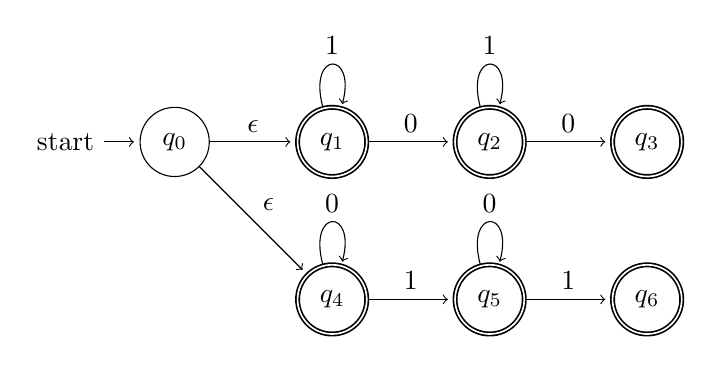
\begin{tikzpicture}[shorten >=2pt,node distance=2cm,on grid,auto]
            \node[state, initial] (q_0)   {$q_0$};
            \node[state, accepting, semithick] (q_1) [right=of q_0] {$q_1$};
            \node[state, accepting, semithick] (q_2) [right=of q_1] {$q_2$};
            \node[state, accepting, semithick] (q_3) [right=of q_2] {$q_3$};
            \node[state, accepting, semithick] (q_4) [below=of q_1] {$q_4$};
            \node[state, accepting, semithick] (q_5) [right=of q_4] {$q_5$};
            \node[state, accepting, semithick] (q_6) [right=of q_5] {$q_6$};
            \path[->]
                (q_0)
                    edge node {$\epsilon$} (q_1)
                    edge node {$\epsilon$} (q_4)
                (q_1)
                    edge [loop above] node {1} (q_1)
                    edge node {0} (q_2)
                (q_2)
                    edge [loop above] node {1} (q_2)
                    edge node {0} (q_3)
                (q_4)
                    edge [loop above] node {0} (q_4)
                    edge node {1} (q_5)
                (q_5)
                    edge [loop above] node {0} (q_5)
                    edge node {1} (q_6);
        \end{tikzpicture}
    \end{figure}

    \textbf{Justification}
    \\

    $q_0$ initiates two branches: one that restricts the number of 0's in the string, 
    and one that restricts the number of 1's. If the string contains $\leq2$ instances of 0 or 1,
    then at least one branch will end on an accept state. If both branches detect $>2$ 0's and 1's,
    the branches will crash on $q_3$ and $q_6$.
    \\

    \textbf{Part Three}

    \begin{figure}[h]
        \centering
        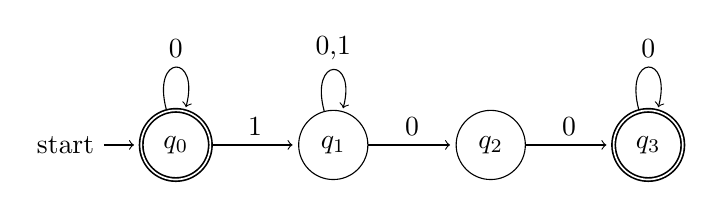
\begin{tikzpicture}[shorten >=2pt,node distance=2cm,on grid,auto]
            \node[state, initial, accepting, semithick] (q_0)   {$q_0$};
            \node[state] (q_1) [right=of q_0] {$q_1$};
            \node[state] (q_2) [right=of q_1] {$q_2$};
            \node[state, accepting, semithick] (q_3) [right=of q_2] {$q_3$};
            \path[->]
                (q_0)
                    edge [loop above] node {0} (q_0)
                    edge node {1} (q_1)
                (q_1)
                    edge [loop above] node {0,1} (q_1)
                    edge node {0} (q_2)
                (q_2)
                    edge node {0} (q_3)
                (q_3)
                    edge [loop above] node {0} (q_3);
        \end{tikzpicture}
    \end{figure}

    \textbf{Justification}
    \\

    Binary multiples of 4 are either a string of all 0's, or a string containing at least
    one 1 where the last two bits are 0's. $q_0$ covers the first case, and also accomodates
    for any 0's at the beginning of our nonzero multiple of 4. If our thread is at $q_1$,
    we only want to accept zero or more 0's or 1's, strictly followed by two 0's. The logic
    for this segment of the NFA is similar to that in part one.
    \\

\end{homeworkProblem}


\begin{homeworkProblem}
    Via subset construction, provide the corresponding DFAs for the problem 1 NFAs.

    \textbf{Solution}
    \\
    \\
    \\
    \textbf{Part One}

    \begin{table}[ht]
        \centering
        \begin{tabular}{c || c | c}
            State
            & $0$
            & $1$
            \\
            \hline
            $q_0$ & $q_0$ & $\{q_0, q_1\}$ \\
            $\{q_0, q_1\}$ & $\{q_0, q_2\}$ & $\{q_0, q_1, q_2\}$ \\
            $\{q_0,q_2\}$ & $\{q_0,q_3\}$ & $\{q_0,q_1,q_3\}$ \\
            $\{q_0, q_1, q_2\}$ & $\{q_0, q_2, q_3\}$ & $\{q_0,q_1,q_2,q_3\}$ \\
            $\{q_0,q_3\}$ & $q_0$ & $\{q_0,q_1\}$ \\
            $\{q_0,q_1,q_3\}$ & $\{q_0,q_2\}$ & $\{q_0,q_1\}$ \\
            $\{q_0,q_2,q_3\}$ & $\{q_0,q_3\}$ & $\{q_0,q_1,q_3\}$ \\
            $\{q_0,q_1,q_2,q_3\}$ & $\{q_0,q_2,q_3\}$ & $\{q_0,q_1,q_2,q_3\}$ \\ 
        \end{tabular}
    \end{table}

    \begin{figure}[h]
        \centering
        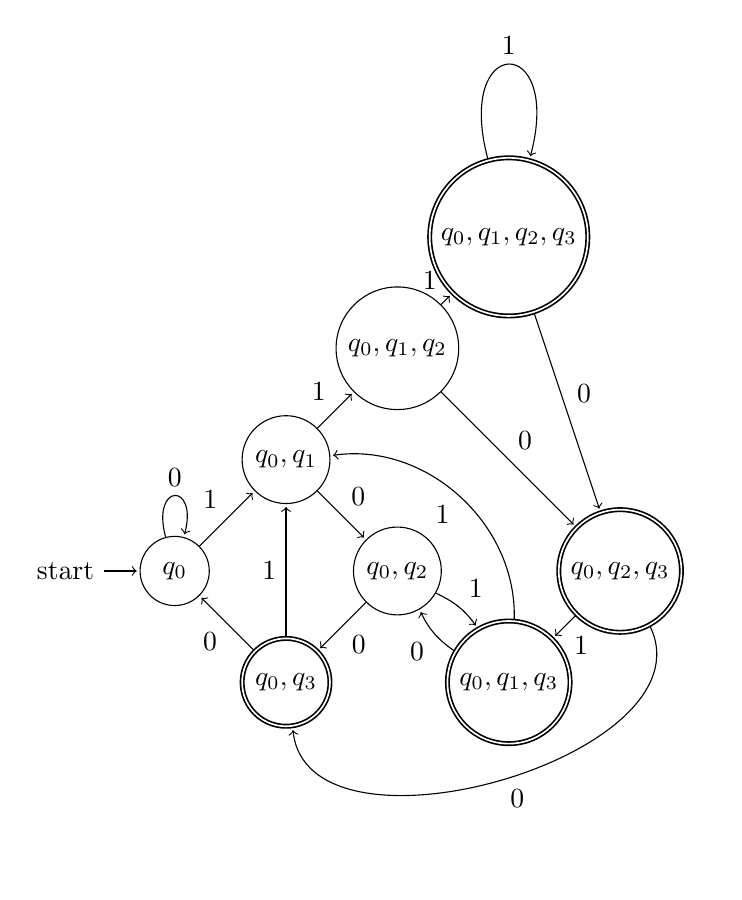
\begin{tikzpicture}[shorten >=1pt,node distance=2cm,on grid,auto]
            \node[state, initial] (q_0)   {$q_0$};
            \node[state] (q_0_1) [above right=of q_0] {$q_0,q_1$};
            \node[state] (q_0_2) [below right=of q_0_1] {$q_0,q_2$};
            \node[state] (q_0_1_2) [above right=of q_0_1] {$q_0,q_1,q_2$};
            \node[state, accepting, semithick] (q_0_3) [below left=of q_0_2] {$q_0,q_3$};
            \node[state, accepting, semithick] (q_0_1_3) [below right=of q_0_2] {$q_0,q_1,q_3$};
            \node[state, accepting, semithick] (q_0_2_3) [above right=of q_0_1_3] {$q_0,q_2,q_3$};
            \node[state, accepting, semithick] (q_0_1_2_3) [above right=of q_0_1_2] {$q_0,q_1,q_2,q_3$};
            
            \path[->]
                (q_0)
                    edge [loop above] node {0} (q_0)
                    edge node {1} (q_0_1)
                (q_0_1)
                    edge node {0} (q_0_2)
                    edge node {1} (q_0_1_2)
                (q_0_2)
                    edge node {0} (q_0_3)
                    edge [bend left=15] node {1} (q_0_1_3)
                (q_0_1_2)
                    edge node {0} (q_0_2_3)
                    edge node {1} (q_0_1_2_3)
                (q_0_3)
                    edge node {0} (q_0)
                    edge node {1} (q_0_1)
                (q_0_1_3)
                    edge [bend left=15] node {0} (q_0_2)
                    edge [bend right=50] node {1} (q_0_1)
                (q_0_2_3)
                    edge [bend left=100] node {0} (q_0_3)
                    edge node {1} (q_0_1_3)
                (q_0_1_2_3) 
                    edge node {0} (q_0_2_3)
                    edge [loop above] node {1} (q_0_1_2_3);
        \end{tikzpicture}
    \end{figure}

    \textbf{Part Two}
    \\
    \begin{table}[ht]
        \centering
        \begin{tabular}{c || c | c}
            State
            & $0$
            & $1$
            \\
            \hline
            $q_0$ & $\{q_2,q_4\}$ & $\{q_1, q_5\}$ \\
            $\{q_2,q_4\}$ & $\{q_3,q_4\}$ & $\{q_2,q_5\}$ \\
            $\{q_1,q_5\}$ & $\{q_2,q_5\}$ & $\{q_1,q_6\}$ \\
            $\{q_3,q_4\}$ & $q_4$ & $q_5$ \\
            $\{q_2,q_5\}$ & $\{q_3,q_5\}$ & $\{q_2,q_6\}$ \\
            $\{q_1,q_6\}$ & $q_2$ & $q_1$ \\
            $q_4$ & $q_4$ & $q_5$ \\
            $q_5$ & $q_5$ & $q_6$ \\
            $\{q_3,q_5\}$ & $q_5$ & $q_6$ \\
            $\{q_2,q_6\}$ & $q_3$ & $q_2$ \\
            $q_2$ & $q_3$ & $q_2$ \\
            $q_1$ & $q_2$ & $q_1$ \\
            $q_6$ & $\emptyset$ & $\emptyset$ \\
            $q_3$ & $\emptyset$ & $\emptyset$ \\
            $\emptyset$ & $\emptyset$ & $\emptyset$ \\
        \end{tabular}
    \end{table}

    \begin{figure}[h]
        \centering
        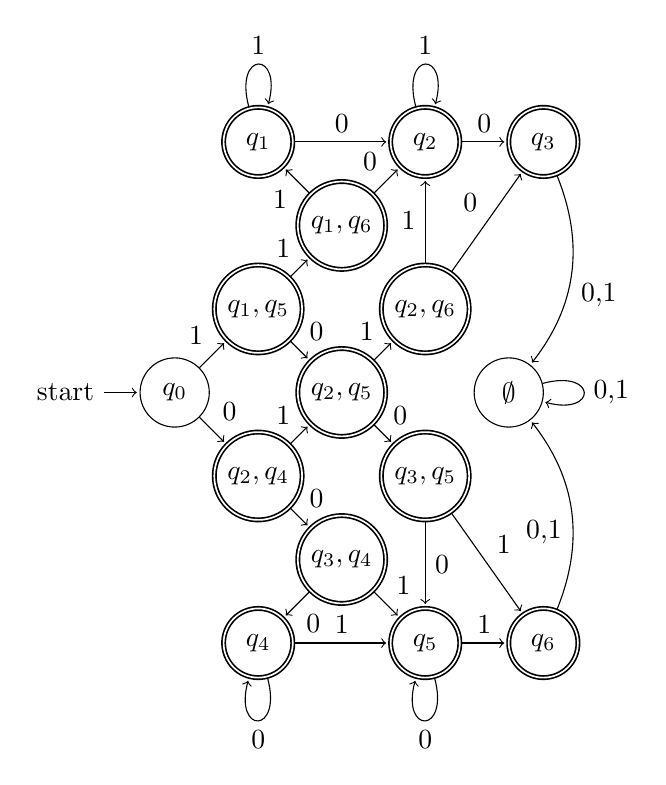
\begin{tikzpicture}[shorten >=1pt,node distance=1.5cm,on grid,auto]
            \node[state, initial] (q_0) {$q_0$};
            \node[state, accepting, semithick] (q_2_4) [below right=of q_0] {$q_2,q_4$};
            \node[state, accepting, semithick] (q_1_5) [above right=of q_0] {$q_1,q_5$};
            \node[state, accepting, semithick] (q_3_4) [below right=of q_2_4] {$q_3,q_4$};
            \node[state, accepting, semithick] (q_2_5) [above right=of q_2_4] {$q_2,q_5$};
            \node[state, accepting, semithick] (q_1_6) [above right=of q_1_5] {$q_1,q_6$};
            \node[state, accepting, semithick] (q_4) [below left=of q_3_4] {$q_4$};
            \node[state, accepting, semithick] (q_5) [below right=of q_3_4] {$q_5$};
            \node[state, accepting, semithick] (q_3_5) [below right=of q_2_5] {$q_3,q_5$};
            \node[state, accepting, semithick] (q_2_6) [above right=of q_2_5] {$q_2,q_6$};
            \node[state, accepting, semithick] (q_1) [above left=of q_1_6] {$q_1$};
            \node[state, accepting, semithick] (q_2) [above right=of q_1_6] {$q_2$};
            \node[state, accepting, semithick] (q_6) [right=of q_5] {$q_6$};
            \node[state, accepting, semithick] (q_3) [right=of q_2] {$q_3$};
            \node[state] (null) [below right=of q_2_6] {$\emptyset$};
            \path[->]
                (q_0)
                    edge node {0} (q_2_4)
                    edge node {1} (q_1_5)
                (q_2_4)
                    edge node {0} (q_3_4)
                    edge node {1} (q_2_5)
                (q_1_5)
                    edge node {0} (q_2_5)
                    edge node {1} (q_1_6)
                (q_3_4)
                    edge node {0} (q_4)
                    edge node {1} (q_5)
                (q_2_5)
                    edge node {0} (q_3_5)
                    edge node {1} (q_2_6)
                (q_1_6)
                    edge node {0} (q_2)
                    edge node {1} (q_1)
                (q_4)
                    edge [loop below] node {0} (q_4)
                    edge node {1} (q_5)
                (q_5)
                    edge [loop below] node {0} (q_5)
                    edge node {1} (q_6)
                (q_3_5)
                    edge node {0} (q_5)
                    edge node {1} (q_6)
                (q_2_6)
                    edge node {0} (q_3)
                    edge node {1} (q_2)
                (q_2)
                    edge node {0} (q_3)
                    edge [loop above] node {1} (q_2)
                (q_1)
                    edge node {0} (q_2)
                    edge [loop above] node {1} (q_1)
                (q_3)
                    edge [bend left] node {0,1} (null)
                (q_6)
                    edge [bend right] node {0,1} (null)
                (null)
                    edge [loop right] node {0,1} (null);
        \end{tikzpicture}
    \end{figure}
    \pagebreak
    \textbf{Part Three}
    \\
    \begin{table}[ht]
        \centering
        \begin{tabular}{c || c | c}
            State
            & $0$
            & $1$
            \\
            \hline
            $q_0$ & $q_0$ & $q_1$ \\
            $q_1$ & $\{q_1,q_2\}$ & $q_1$ \\
            $\{q_1,q_2\}$ & $\{q_1,q_2,q_3\}$ & $q_1$ \\
            $\{q_1,q_2,q_3\}$ & $\{q_1,q_2,q_3\}$ & $q_1$ \\

        \end{tabular}
    \end{table}
    \begin{figure}[h]
        \centering
        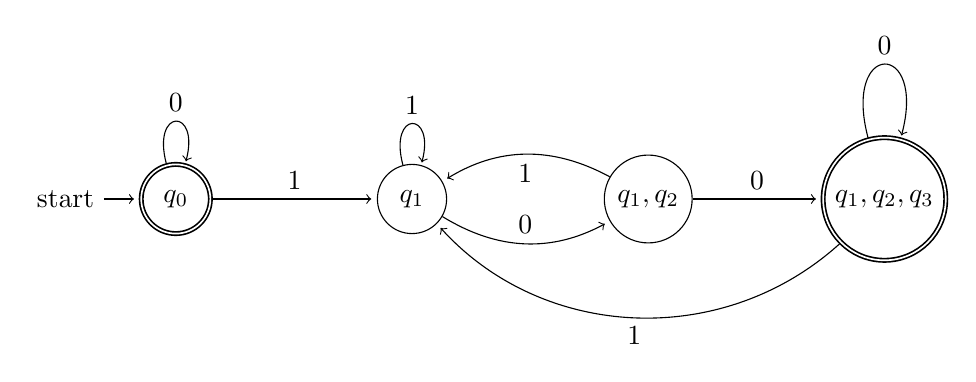
\begin{tikzpicture}[shorten >=2pt,node distance=3cm,on grid,auto]
            \node[state, initial, accepting, semithick] (q_0)   {$q_0$};
            \node[state] (q_1) [right of=q_0] {$q_1$};
            \node[state] (q_1_2) [right of=q_1] {$q_1,q_2$};
            \node[state, accepting, semithick] (q_1_2_3) [right of=q_1_2] {$q_1,q_2,q_3$};
            \path[->]
                (q_0)
                    edge [loop above] node {0} (q_0)
                    edge node {1} (q_1)
                (q_1)
                    edge [bend right] node {0} (q_1_2)
                    edge [loop above] node {1} (q_1)
                (q_1_2)
                    edge node {0} (q_1_2_3)
                    edge [bend right] node {1} (q_1)
                (q_1_2_3)
                    edge [loop above] node {0} (q_1_2)
                    edge [bend left=45] node {1} (q_1);
        \end{tikzpicture}
    \end{figure}

    




\end{homeworkProblem}
\end{document}